\newcommand{\Cont}{\mathcal{C}}%
\section{Notation}
Let $X$ be a set. We will denote by $X^\star$ the set of all finite sequence with elements in $X$.

\section{Introduction}
In abstraction of dynamical systems, the knowledge of the sequence of inputs applied to the plant might sometimes be preferable than the knowledge of the full state.
%
%The transient states of the system make the control synthesis more complex in some situation (small environment, or noisy environment).
%More accurate models (second integrator with a small discretization of the state space) could be used with some drawbacks on the complexity and on the computation time.
Hereby we present an abstraction of a dynamical model (discrete or continuous time) obtained by extending the state with the knowledge of the finite time input sequence lastly applied to the system.
We have successfully used this abstraction in order to control quadricopters. Abstraction obtained were a good alternative to solve the controller synthesis while keeping the complexity acceptable.


% Property that needs to be verified by the abstraction
In the next parts, this abstraction will be used in order to find a controller for the system.
If the system and the abstraction verify a relation (alternating simulation relation), then any property verify by the controlled abstraction will be verified as well by the controlled system with the same controller.


\section{Related work}
Talk about formal verifications methods.

The needs of discrete abstraction.


\section{Preliminaries}
%% MOVE THIS PART
In \cite{tabuada2009verification}, the link between in hybrid systems is investigated. 
\begin{nameddef}{System}\label{def:system}
$S = (X,X_0,\U, \systransition{S}{}, Y,H)$
where:
\begin{itemize}[noitemsep,nolistsep]
\item $X$ is a set of states;
\item $X_0 \subset X$ a set of initial states;
\item $\U$ a set of inputs;
\item $\systransition{S}{} \subseteq X \times \U \times X$ a transition relation ;
\item $Y$ a set of outputs;
\item $H:X \rightarrow Y$ an output map.\popQED
\end{itemize}
\end{nameddef}

This definition of system cover both the discrete and continuous time case of dynamical systems.
For the continuous case, the time variable is included as part of the set of inputs.
Let $\traj$ be the trajectory function of the dynamical system.
A transition of the dynamical system from $\x$ at $t$ to $\x'= \traj(t_0,\x,\u)$ at $t+t_0$  will be written: $$\x \systransition{S}{t_0,\u} \x'$$.
For the discrete case, a transition correspond to 1 timestep.
The sets of states and of inputs does not have to verify any specific property, they can be infinite of finite sets.

Note: in the future we will use a second equivalent notations for the transition relation $\systransition{S}{\u}$ of a system $S$: $\Post{S}{\u}$  defined for $\x \in X$ and $\u \in \U$ by:
\begin{equation}
\Post{S}{\u}(\x) = \{ \x' \in X \mid \x \systransition{S}{\u} \x' \}
\end{equation}
This definition correspond to the set of all the successors of the state $\x$ after applying $\u$.

The alternating simulation relation between 2 systems is the link between discrete abstraction and the continuous representation of this system.
For commodity, the definition of alternative simulation is rewritten here (\cite{tabuada2009verification}):
\begin{nameddef}{Alternating simulation} \label{def_alt_sim}
Let $\sysA$ and $\sysB$ 2 systems with $Y_a=Y_b$, $\sysA$ is alternatingly simulated by $\sysB$ (noted $\sysA \altsim \sysB$)if there exists a relation $R \subseteq X_a \times X_b$ that verify:
\begin{enumerate}[noitemsep,nolistsep]
\item $\forall x_{a0} \in X_{a0}, \exists x_{b0} \in X_{b0}, (x_{a0},x_{b0}) \in R$
\item $\forall (x_a,x_b) \in R, H_a(x_a) = H_b(x_b)$
\item $\forall (x_a,x_b) \in R, \forall u_{a} \in \U_{a}, \exists u_{b} \in \U_{b}$\\
$\forall x_b' \in \Post{\sysB}{u_b}(x_b),\exists x_a' \in \Post{\sysA}{u_a}(x_a), (x_a',x_b') \in R$
\popQED
\end{enumerate}
\end{nameddef}
This is important to note that this relation is commuting: for 3 systems $\sysA$,$\sysB$ and $\sysC$, if $\sysA \altsim \sysB$ and $\sysB \altsim \sysC$, then $\sysA \altsim \sysC$. This property will be used in the construction of the abstraction where several transformations will be used before getting the final transformation.
\comment{I need to write the property saying why this definition is nice (behavioural), or at least explain it and then refer to the book of tabuada}


%% INPUT SEQUENCE REACHABLE SETS
In the next sections, we will focus on systems with input memories. The knowledge of unobserved variables will be replaced by computation of reachable sets thanks to the last input sequence $\Pastuseq$.
The reachable sets will have an analytical form for simpler models. We would like first to give a general definitions of these sets.
First we define the reachable sets for a fully known sequence of controls, then for a the last $n$ inputs applied to the system.
For a system $S$, let $\Reach{S}{U} \subseteq X$ defined for a finite sequence $U \in \U^\star$ of $N \in \mathbb{N}$ control actions by:
\begin{equation}
\begin{split}
\x \in \Reach{S}{U}
\Leftrightarrow &
\exists \x_0 \in X_0,
\forall i<N,i>0, \exists \x_i \in X,\\
&\x_0 \systransition{S}{\u_0} \x_1
\systransition{S}{\u_1} \dots
\systransition{S}{\u_{N-1}} \x
\end{split}
\end{equation}
$\Reach{S}{U}$ correspond to all the reachable states with the sequence inputs $U$.

%% Define the reached states:
\renewcommand{\v}{\vect{v}}
\newcommand{\useq}{\v_{1-n},\dots,\v_{0}}
\begin{definition}
For a finite sequence $\Pastuseq = \left\{ \useq \right\}$ of $n$ controls in $\U$,
let $X(\Pastuseq) \subseteq X$ the set of all the states reached by a control sequence terminating with $\Pastuseq$:
\begin{equation}
\ReachSeq{S}{\Pastuseq}
=
\bigcup_{\{\vu_i\}_{i < \infty} \in \U^\star}
\Reach{S}{\{\vu_0,\vu_1,\dots,\useq\}}
\end{equation}
\end{definition}

\section{Abstraction} \label{sec:abstraction}
%
The creation of the abstraction is done in the following steps (summarized in \ref{proc_abstraction}):
\begin{itemize}[noitemsep,nolistsep]
\item $S \rightarrow S':$ we first create the system with a state extended by a sequence of inputs,
\item $S' \rightarrow S_a:$ then we project the output set to only partially observe the state, the removed information is "replaced" by computation of reachable sets,
\item $S_a \rightarrow S_a':$ finally, the state space is discretized.
\end{itemize}

We will see that there is no alternating simulation relation between $S$ and $S'$ mainly for technical reasons that does not affect the rest of the abstraction computation. The 2 last transformations will need the alternating simulation relations to make possible the controller synthesis over the system $S'$.

\begin{figure}
\includestandalone[width=\linewidth]{abstraction_process}
\caption{Steps to create the abstraction}
\label{proc_abstraction}
\end{figure}

\subsection{$S \rightarrow S'$}
Let the system $\sys = (\tuple{X,X_0,\U,\systransition{S}{},Y,H})$
and the same system with a state extended by memories of the last $\Ninputs$ control actions applied to the system, $\sys'$ defined by
$\sys' =  (\tuple{X',X_{0}',\U,\systransition{S'}{},Y',H'})$ 
where:
\begin{itemize}[nolistsep,noitemsep]
\item $X' = X \times \U^{\Ninputs}$ the set of states, 
\item $X_{0}' = X_0 \times \U^{\Ninputs}$ the set of initial states,
\item $Y' = Y \times \U^{\Ninputs}$ the set of outputs,
\item $H'$ the output map defined for all $(x,\Pastuseq) \in X'$ as $H'(x') = (H(x),\Pastuseq)$
\item and the transition relation defined by:
\begin{equation}
\begin{split}
(\x,\u_{n - \Ninputs},...,\u_{n-1}) 
\systransition{S'}{\u} &
 (\x',\u_{n+1-\Ninputs},...,\u_{n-1},\u)\\
\Longleftrightarrow 
&
\left\{
\begin{split}
&\x \systransition{S}{\u} \x' \\
&\x \in \ReachSeq{S}{\u_{n - \Ninputs},...,\u_{n-1}}
\end{split}
\right.
\end{split}
\end{equation}
\end{itemize}
As the system $S$ and the system $S'$ do not have the same set of outputs, it is not possible to find an alternating simulation relation between the 2 systems.
This has further implications: the controller synthesis will not be applicable for $S$ but only for $S'$ as the controller solution for $S'$ cannot be composed with the system $S$.
However, we found interesting to perform this first transformation from $S$ to $S'$ to underline the key difference between the 2 systems (apart from the state extension): for a sequence of inputs, all the states that are not reachable has been suppressed.
We do not lose any crucial information as all the trajectories of the system $S$ are in the system $S'$ and vice versa.

\subsection{$S' \rightarrow S_a$}
In this part, we change the state of the system by considering only a subspace of it.
To counteract the loss of information, we have to find a set of the possible unobserved states.
This is done by computation of reachable sets out of the sequence of inputs (that is part of the state).

We will assume that the state $\x$ of the system $\sys$ can be decomposed in this way $\displaystyle\T{\x} = \T{[\T{\xobs},\T{\xunobs}]}$ where $\xobs \in Y$  is observed and $\xunobs$ is an unobserved (internal) state.
Lets call $\SSunobs$ the subspace of $\xunobs$ and $\SSobs$ the one of $\xobs$.
The states of the input extended state abstraction $\sysa$ will be expressed by $\xa_n = (\xobs_n,\Pastuseq)$ where $\Pastuseq = [\pastuseq] \in \U^{\Ninputs}$.

Let the set
$$\Xunobs(\Pastuseq) = \Reach{S}{\Pastuseq} \proj{\SSunobs}$$.
$\Xunobs(\Pastuseq)$ correspond to all the unobserved states that can be reached by the system $S'$ after applying a control sequence terminating with $\Pastuseq$.
We can now "replace" the knowledge of the state  $\xunobs$ by the set of all the possible states $\Xunobs(\Pastuseq)$.
% Definition of the reduced system
Let the system
$\sysa =  (X_a,X_{a 0}, \sysaU, \transition, Y_a, H_a)$ 
where:
\begin{itemize}[nolistsep,noitemsep]
\item $X_a = \Xobs \times \sysaU^{\Ninputs}$ the set of states, 
\item $X_{a 0} = \Xobsinit \times  \mathcal{U}^{\Ninputs}$ the set of initial states,
\item $Y_a = Y'$ the set of outputs,
\item $H_a$ the output map defined for $\xa = (\xobs,\Pastuseq) \in X_a$ by $H_a(\xa) = (\xobs,\Pastuseq)$,
\item and the transition relation is defined by:
\begin{equation}
\begin{split}
(\xobs_n,\vect{u}_{n - \Ninputs},...,\vect{u}_{n-1}) 
\labelledtransition{\vu} 
& (\xobs_{n+1},\vect{u}_{n+1-\Ninputs},...,\vect{u}_{n-1},\vu)\\ \Longleftrightarrow 
\xobs_{n+1} \in 
& H_a(Post^S_{\vu}(\{\xobs\} \times \Xunobs(\vect{u}_{n - \Ninputs},...,\vect{u}_{n-1}))
\end{split}
\end{equation}
\end{itemize}

%% MISSING PROOF THAT IT IS AN ALTERNATING SIMULATION RELATION
\begin{prop}
$\sysa$ is alternatingly simulated by $\sys'$ ($S_a \altsim S'$).
\end{prop}

\begin{proof}
Let $R$ the relation defined by:
\begin{equation}
R = \{ (\x',\xa) \in X' \times X_a \mid H'(\x') = H_a(\xa) \}
\end{equation}
By definition of the systems $S'$, $\sysa$ and of the relation $R$, conditions 1 and 2 of definition \ref{def_alt_sim} are already verified.

In order to prove that condition 3 lie, it is sufficient to show that the unobserved part of $\x$ is contained in the set $\Xunobs(\Pastuseq)$.

Let $(\x',\xa) \in R$, $\u \in U$ and $\x'_+ \in \Post{S'}{\u}(\x')$.
As $H'(\x') = H_a(\xa)$, $\x' \proj{\U^\Ninputs} = \xa \proj{\U^\Ninputs}$, to put this in words, the states have the same past inputs, we will denote this sequence with $\Pastuseq$.
By definition of $\Xunobs(\Pastuseq)$,
we know that $\x' \proj{\SSunobs} \in \Xunobs(\Pastuseq)$,
so
$\x' \in \{\x' \proj{\SSobs} \} \times \Xunobs(\Pastuseq) \times \Pastuseq$
which imply that
$\x'_+ \in \Post{S'}{\u}(\{\x' \proj{\SSobs} \} \times \Xunobs(\Pastuseq) \times \Pastuseq )$.
By taking $\xa_+ = H_a(\x'_+) \in \Post{S_a}{\u}(\xa)$,
we have $(\x'_+,\xa_+) \in R$.
\end{proof}

\subsection{$S_a \rightarrow S_a'$}
In order to apply computer science tools, we would like to have an abstraction with finite state space and finite input space.
In order to have this, we will discretize both of them.

\newcommand{\symbD}{P}
\newcommand{\setD}{\mathcal{P}}
\newcommand{\sizeD}{\mathcal{I}}
We first define the discretization of the state space.
Let $\symbD_i$ a finite set of symbols associated with the finite set of subsets $\setD_i \subset X_a$ for $i>\sizeD \in \mathbb{N}$ so that:
\begin{equation}
\begin{split}
&\bigcap_{0 \leq i < \sizeD} \setD_i = X_a \\
&\forall i,j< \sizeD,0<i,j, \setD_i \cap \setD_j = \emptyset\\
\end{split}
\end{equation}
\newcommand{\symbU}{V}
\newcommand{\setU}{\mathcal{V}}
\newcommand{\sizeU}{\mathcal{J}}
We define in the same way the discretization of the input space. 
Let $\symbU_i$ a finite set of symbols associated with the finite set of subsets $\setU_i \subset X_a$ for $i>\sizeU \in \mathbb{N}$ so that:
\begin{equation}
\begin{split}
&\bigcap_{0 \leq i < \sizeU} \setU_i = \U \\
&\forall i,j< \sizeU,0<i,j, \setU_i \cap \setU_j = \emptyset\\
\end{split}
\end{equation}

\newcommand{\symbO}{P^o}
\newcommand{\setO}{\mathcal{P}^o}
\newcommand{\sizeO}{\mathcal{K}}
We will use the same discretization for the observed variable and the state space projected on the observed space. The notation will be $\symbO$ for the symbols,$\setO$ for the sets and $\sizeO$ for the number of elements.

The final abstraction is then defined in this way. Let the system $S_a' = (\tuple{X_a',X_{a 0}', U', \systransition{S_a'}{}, Y_a', H_a'})$ defined by:
\begin{itemize}[nolistsep,noitemsep]
\item $X_a' = \{\symbD_1,\dots,\symbD_\sizeD\}$ the set of states, 
\item $X_{a 0}' \subseteq X_a'$ the set of initial states defined for $i$, $\symbD_i \in X_{a 0}' \Leftrightarrow \setD_i \cap X_{a 0} \neq \emptyset$,
\item $Y_a' = \{\symbO_1,\dots,\symbO_\sizeO\}$ the set of outputs,
\item $H_a'$ the output map defined for $\symbD_i = \in X_a'$ by $H_a(\symbD_i)$ the only symbol $\symbO_j$ in $Y_a'$ so that $\setD_i |_{\SSobs} = \setO_j$ (by shoosing the same discretization than the state space, the existence and unicity is ensured),
\item and the transition relation is defined by:
\begin{equation}
\symbD_i 
\systransition{S_a'}{\u} 
\symbD_j
\Longleftrightarrow 
\exists \xa \in \setD_i, \xa_+ \in \setD_j, 
\xa \systransition{S_a}{\u} \xa_+
\end{equation}
\end{itemize}

The previous definition is using a small abuse of notation: the discretization should have been done in the first place as the chosen output maps now differe from the initial system, however, this does not change the rest of the proof.
The alternating simulation relation is ensured by the fact that we are doing over approximation of the state through the discretization. So we have $S_a \altsim S_a'$.

As the relation $\altsim$ is commuting, we have the following property:
$S_a' \altsim S'$. This is the main property that we needs in order to use this abstraction for the controller synthesis.


\comment{You need to see with PJ how to go for this part, when do I need to introduce the symbols because right now $S_a$ and $S_a'$ have different output maps. So I need to have a more uniform approach there.}

\section{Dynamical systems}
As the definition \ref{def:system} of a system can be used in order to represent continuous and discrete dynamical systems.
In this case, the computation of the sets $\Xunobs(\Pastuseq)$ is a reachability problem.
It can be solved in 2 steps: find the smallest invariant $\Xuinv$ of $\sys$ dynamics on $\xunobs$ and compute the image $\Xunobs(\Pastuseq)$ of $\Xuinv$ after applying a control sequence that terminate with $\Pastuseq$.

\begin{figure}
\centering
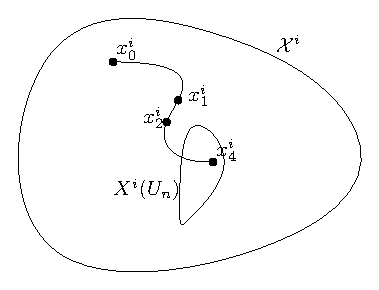
\includegraphics[width=0.5\linewidth]{invariant_set}
\caption{The image of the invariant set $\Xuinv$ after applying the control sequence $\Pastuseq$ is $\Xunobs(\Pastuseq)$}
\end{figure}

% Here I am trying to explain why I have been choosing a smaller class of systems
Interesting case scenarios happen when the knowledge about $\Xunobs(\Pastuseq)$ is preferable to the actual observation of the state $\xunobs$.
If $\Xunobs(\Pastuseq)$ is unbounded, the final abstraction might have an infinite number of successors. The impact on our ability to find a solution must be investigated for each systems, however this property is unlikely to be desirable.
We will therefore focus on systems that have bounded invariant sets $\Xuinv$.

From now we will use linear time invariant systems. We use them mainly for their ease of manipulation.